\def\highresexperiments{
    Trước khi bàn luận đến những mô hình giúp giải quyết bài toán object detection trong ảnh chất lượng cao, ta cần xem xét đến vai trò của tỷ lệ giữa kích thước của đối tượng trong ảnh và kích thước ảnh thông qua một số thí nghiệm.
    Cụ thể hơn, nhóm tác giả muốn đánh giá sự ảnh hưởng \textit{domain shift} lên kết quả của mô hình.
    \textit{Domain shift} được định nghĩa là sự thay đổi về tỷ lệ giữa kích thước của đối tượng trong ảnh và kích thước ảnh giữa tập dữ liệu huấn luyện và tập dữ liệu test.
    \textit{Domain shift} rất phổ biến trong bài toán object detection, khi kích thước ảnh sử dụng trong quá trình huấn luyện thường nhỏ (nhằm cải thiện tốc độ huấn luyện mô hình) và kích thước ảnh sử dụng trong quá trình test thường lớn hơn (nhằm cải thiện độ chính xác của mô hình).
    Các thí nghiệm này được xây dựng và công bố kết quả bởi nhóm tác giả của mô hình SNIP \cite{singh2018analysis}.

    \noindent
    \textbf{\textit{Các thí nghiệm trong bài toán image classification}} \\
    Ba mô hình được sử dụng trong các thí nghiệm được thiết kế như sau: \\
    - Mô hình CNN-B: Đây là mô hình CNN sử dụng backbone ResNet-101 và đã được huấn luyện với bộ dữ liệu ảnh có kích thước 224x224. \\
    - Mô hình CNN-S: Đây là mô hình CNN sử dụng backbone ResNet-101 và đã đã được thay đổi các tham số stride và kích thước của conv trong lớp đầu tiên đối với từng bộ dữ liệu ảnh có kích thước khác nhau khi huấn luyện mô hình.
    Khi huấn luyện với bộ dữ liệu ảnh có kích thước 48x48, tác giả dùng conv có kích thước 3x3 và stride bằng 1, khi huấn luyện với bộ dữ liệu ảnh có kích thước 96x96, tác giả dùng conv có kích thước 5x5 và stride bằng 2. \\
    - Mô hình CNN-B-FT: Đây là mô hình CNN sử dụng backbone ResNet-101 và đã được huấn luyện với bộ dữ liệu ảnh có kích thước 224x224 giống như CNN-B.
    Sau đó fine-tune lại với bộ dữ liệu ảnh có kích thước nhỏ hơn nhưng được upsample lên lại kích thước 224x224.

    \begin{figure}[H]
        \centering
        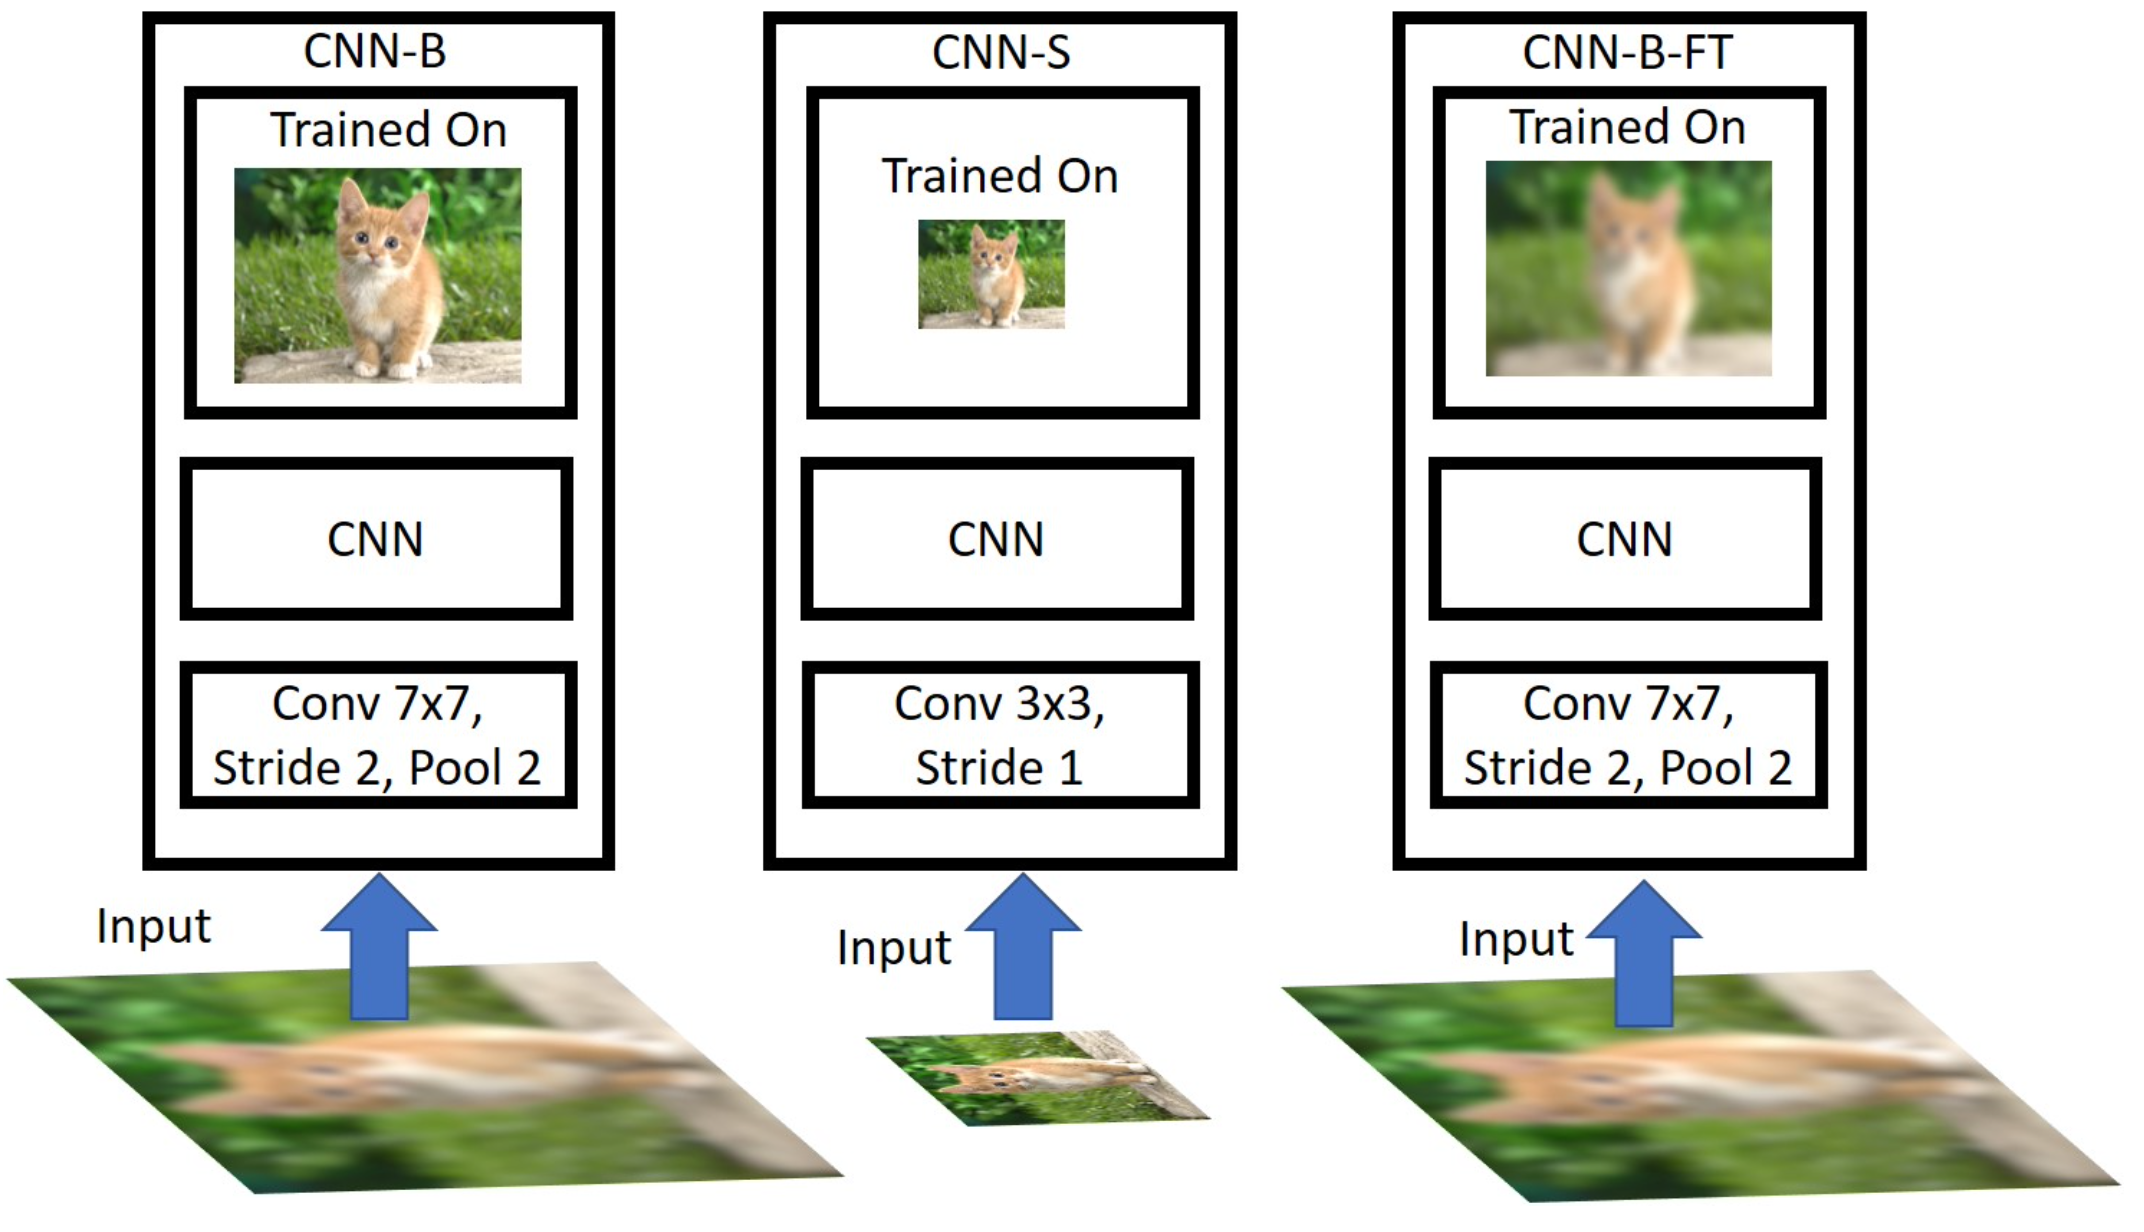
\includegraphics[width=12cm] {images/snip_models_to_exp.png}
        \caption{Ba mô hình được sử dụng trong các thí nghiệm (Nguồn: \cite{singh2018analysis})}
        \label{fig:snip_models_to_exp}
    \end{figure}

    \noindent 
    Nhóm tác giả thực hiện thí nghiệm đầu tiên là \textit{Thí nghiệm Naive Multi-Scale Inference}.
    Nhóm tác giả kiểm tra đánh giá mô hình CNN-B đơn giản với các bộ dữ liệu có kích thước ảnh khác nhau.
    Đầu tiên, nhóm tác giả thu nhỏ kích thước ảnh trong bộ dữ liệu ImageNet từ 224x224 xuống 48x48, 64x64, 80x80, 96x96, 128x128.
    Tiếp theo, nhóm tác giả tăng kích thước ảnh từ 48x48, 64x64, 80x80, 96x96, 128x128 lên lại 224x224.
    Cuối cùng, với các bộ dữ liệu mới nói trên, nhóm tác giả đưa vào mô hình CNN-B và quan sát kết quả.

    \begin{figure}[H]
        \centering
        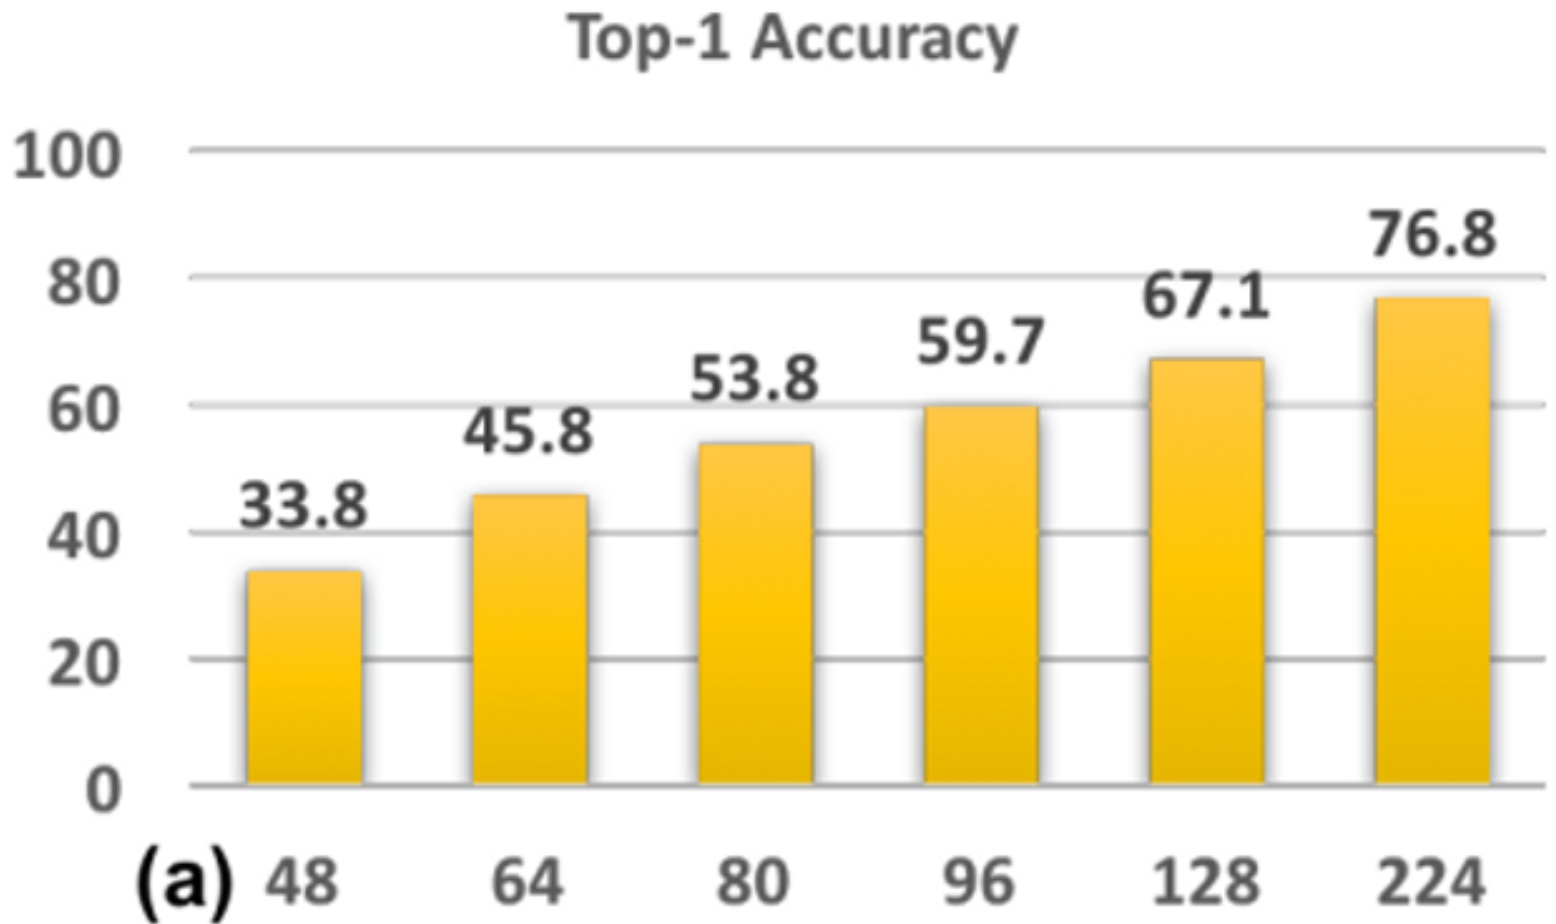
\includegraphics[width=9cm] {images/snip_naive_multi_scale_infer}
        \caption{Kết quả của thí nghiệm Naive Multi-Scale Inference (Nguồn: \cite{singh2018analysis})}
        \label{fig:snip_naive_multi_scale_infer}
    \end{figure}

    \noindent
    \textbf{Kết quả}:
    Ảnh sử dụng trong quá trình huấn luyện và trong quá trình test càng khác nhau về kích thước, khả năng của mô hình càng giảm.
    Cụ thể hơn, kết quả về top-1 accuracy của mô hình CNN-B với các bộ dữ liệu được tăng kích thước từ 48x48, 64x64, 80x80, 96x96, 128x128 lần lượt là 33.8\%, 45.8\%, 53.8\%, 59.7\%, 67.1\%.
    Trong khi đối với bộ dữ liệu được giữ nguyên kích thước 224x224, mô hình CNN-B đạt kết quả 76.8\%. \\
    \textbf{Kết luận}:
    Đối với bài toán classification, việc test mô hình với các kích thước ảnh khác mà mô hình chưa được huấn luyện sẽ gây ra kết quả suy giảm đáng kể.
    Sự chênh lệch càng lớn giữa kích thước ảnh huấn luyện và kích thước ảnh test càng gây ra sự suy giảm kết quả đáng kể.

    \noindent
    Nhóm tác giả thực hiện thí nghiệm thứ hai là \textit{Thí nghiệm Resolution Specific Classifiers}.
    Trong thí nghiệm này, nhóm tác giả thay đổi một chút kiến trúc của mô hình CNN-S.
    Trong kiến trúc của mô hình CNN-B, lớp conv đầu tiên có kích thước stride = 2, và sau đó là lớp max pooling với stride = 2x2.
    Do đó, ngay từ các lớp đầu tiên, các mô hình trên xoá đi các thông tin của các đối tượng nhỏ trong ảnh.
    Từ quan sát trên, nhóm tác giả thay đổi kiến trúc và tạo ra mô hình CNN-S sao cho nó đạt được kết quả tốt nhất trên bộ CIFAR10 (đây là bộ dữ liệu với kích thước ảnh nhỏ).
    Sau đó, nhóm tác giả so sánh kiến trúc của mô hình CNN-S với mô hình CNN-B.

    \begin{figure}[H]
        \centering
        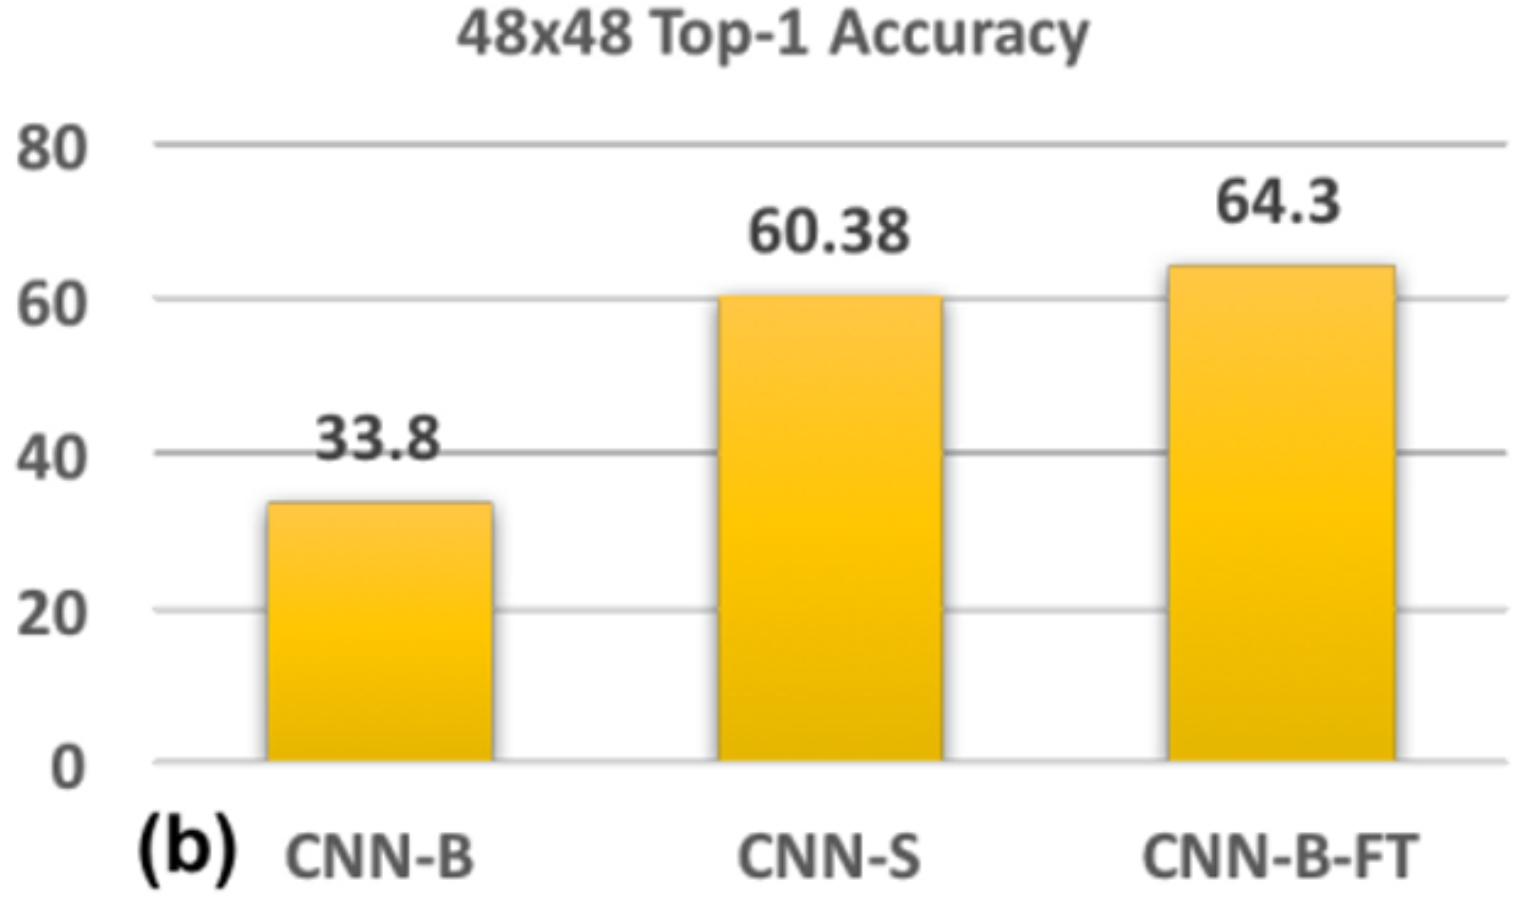
\includegraphics[width=9cm] {images/snip_res_spec_cls}
        \caption{Kết quả của thí nghiệm Resolution Specific Classifiers và Fine-tuning High-Resolution Classifiers trên bộ dữ liệu ảnh có kích thước 48x48 (Nguồn: \cite{singh2018analysis})}
        \label{fig:snip_res_spec_cls}
    \end{figure}

    \noindent
    \textbf{Kết quả}:
    Mô hình CNN-S đạt kết quả tốt hơn rất nhiều so với kết quả của mô hình CNN-B khi xử lý ảnh 48x48.
    Trong khi mô hình CNN-B đạt kết quả 33.8\%, mô hình CNN-S đạt kết quả 60.38\%. \\
    \textbf{Kết luận}:
    Việc thay đổi kiến trúc của mô hình sao cho phù hợp giúp cho mô hình học ảnh có resolution nhỏ tốt hơn.

    \noindent
    Nhóm tác giả thực hiện thí nghiệm cuối cùng trong phần này là \textit{Thí nghiệm Fine-tuning High-Resolution Classifiers}.
    Việc thiết kế và huấn luyện mô hình (tương như như phương án của mô hình CNN-S trong thí nghiệm Resolution Specific Classifiers) với mỗi một bộ dữ liệu có kích thước ảnh khác nhau sẽ tốn quá nhiều công sức và tài nguyên tính toán.
    Từ đó, nhóm tác giả đưa ra một giải pháp đơn giản hơn đó là chiến lược xây dựng mô hình CNN-B-FT.

    \begin{figure}[H]
        \centering
        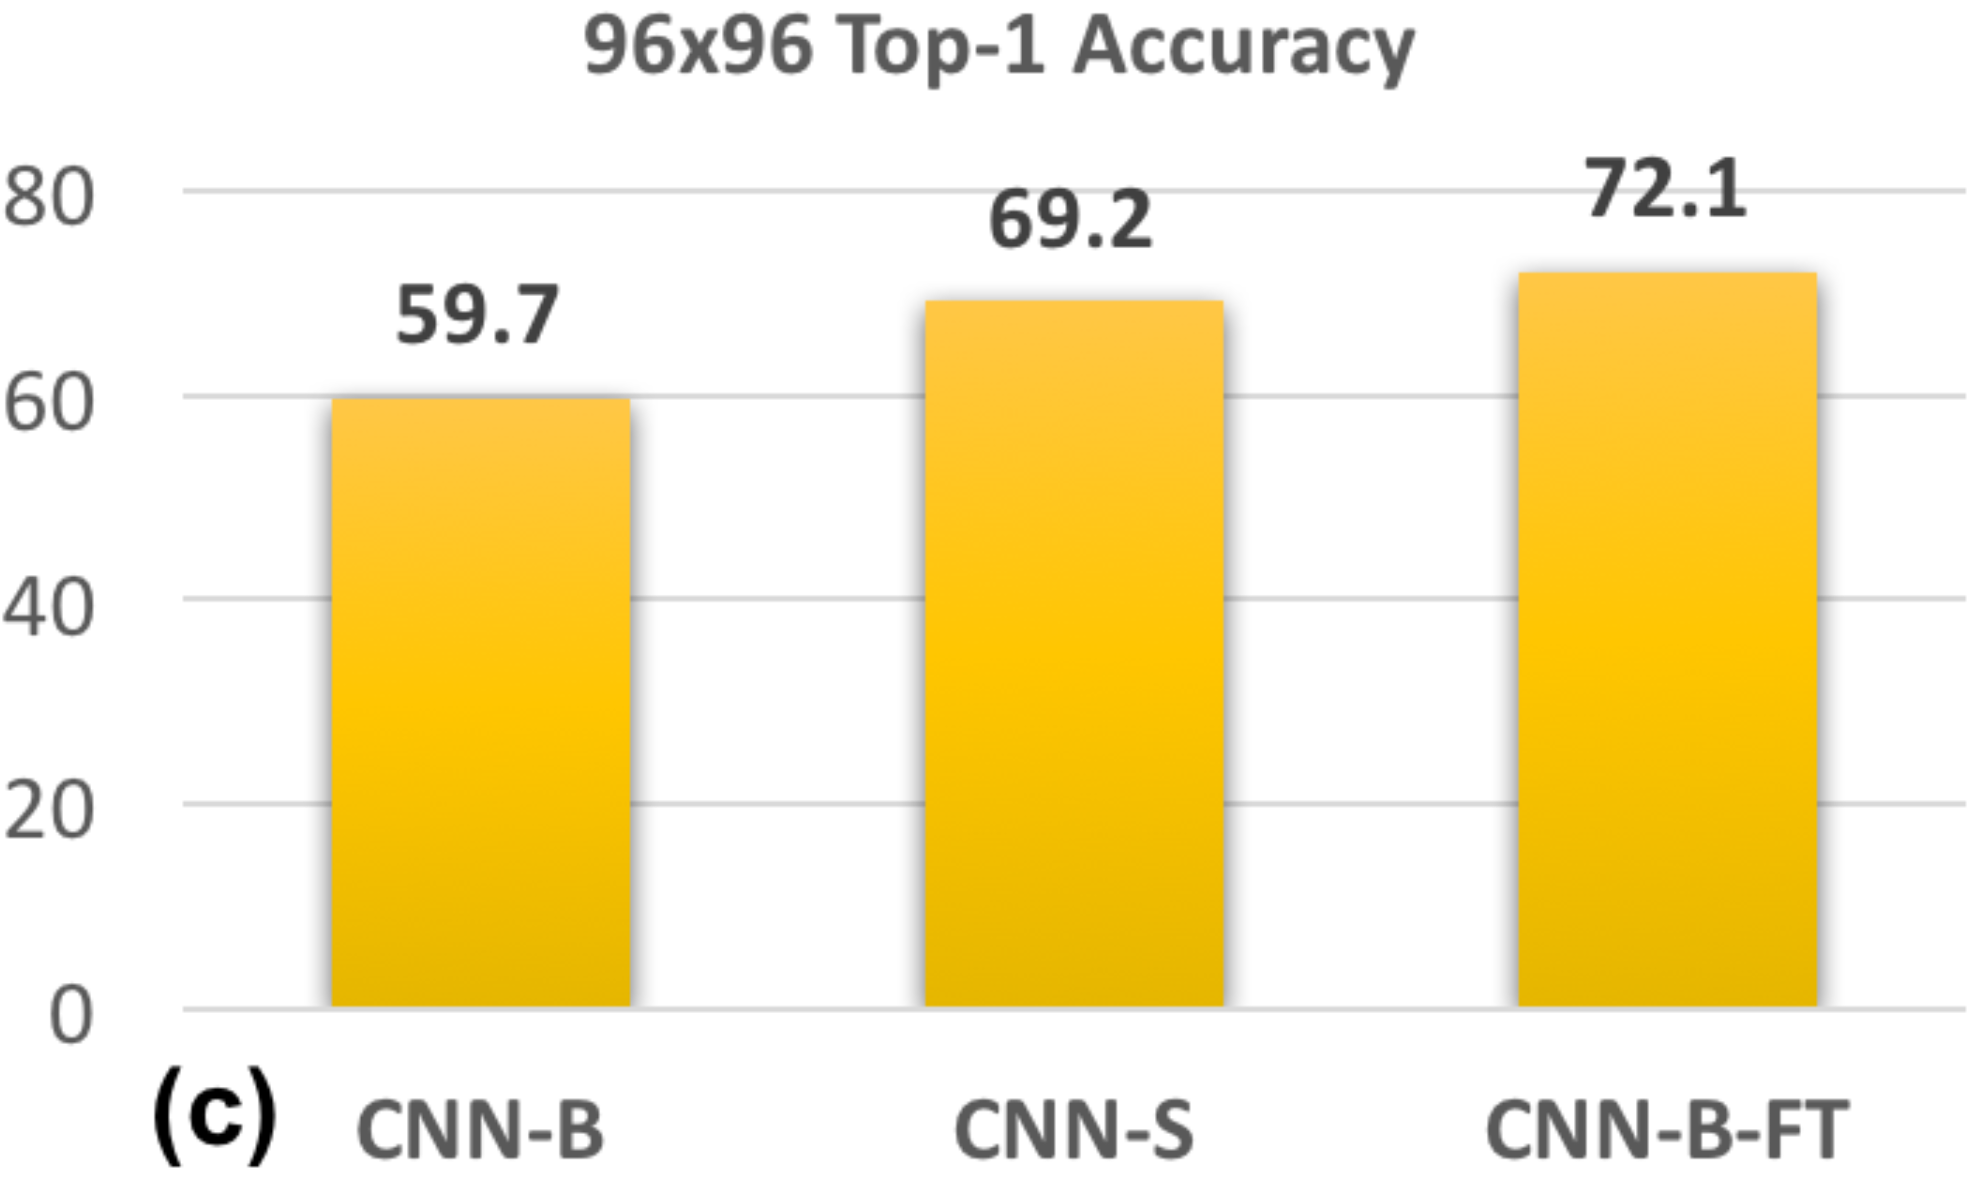
\includegraphics[width=9cm] {images/snip_res_spec_cls_96}
        \caption{Kết quả của thí nghiệm Resolution Specific Classifiers và Fine-tuning High-Resolution Classifiers trên bộ dữ liệu ảnh có kích thước 96x96 (Nguồn: \cite{singh2018analysis})}
        \label{fig:snip_res_spec_cls_96}
    \end{figure}

    \noindent
    \textbf{Kết quả}:
    Mô hình CNN-B-FT có kết quả tốt hơn so với kết quả của mô hình CNN-S. \\
    \textbf{Kết luận}:
    Thí nghiệm trên chứng minh rằng, các trọng số của mô hình CNN-B, được huấn luyện từ bộ dữ liệu ảnh có kích thước lớn, hữu ích trong việc giải quyết bộ dữ liệu ảnh có kích thước nhỏ.
    Từ đó, thay vì giảm kích thước stride của lớp conv đi 2 lần (như trong kiến trúc của mô hình CNN-S), ta nên tăng kích thước của ảnh chất lượng thấp lên lần và fine-tune lại với mô hình đã được huấn luyện với bộ dữ liệu ảnh có kích thước lớn.
    Hay nói cách khác, thay vì thay đổi kiến trúc của mô hình để xử lý riêng với bộ dữ liệu ảnh có kích thước nhỏ, ta nên tận dụng mô hình pretrained và fine-tune lại mô hình đó với bộ dữ liệu ảnh có kích thước mong muốn.

    \noindent
    \textbf{\textit{Các thí nghiệm trong bài toán object detection}} \\
    Hiệu năng giữa các mô hình bị ảnh hưởng bởi sự khác nhau về kích thước của ảnh trong bộ dữ liệu huấn luyện và bộ dữ liệu test đã được nhóm tác giả chứng minh ở các thí nghiệm trên.
    Tuy nhiên, trong thực tế, không phải lúc nào ta cũng có thể huấn luyện và test mô hình với bộ dữ liệu ảnh có cùng kích thước, đặc biệt đối với bài toán object detection.
    Lý do vì những vấn đề liên quan đến bộ nhớ của GPU cũng như là tốc độ huấn luyện, do đó, thông thường kích thước ảnh trong bộ dữ liệu sử dụng trong quá trình huấn luyện thường nhỏ hơn so với kích thước ảnh trong quá trình test.

    \noindent
    Trong các thí nghiệm ở phần này, nhóm tác giả sử dụng chung mô hình là Deformable - RFCN \cite{dai2017deformable}, huấn luyện với những bộ dữ liệu khác nhau nhưng cùng test trên bộ dữ liệu có kích thước 1400x2000 nhằm mục đích đánh giá hiệu năng trong việc xác định các đối tượng nhỏ (kích thước nhỏ hơn 32x32).

    \noindent
    Nhóm tác giả thực hiện thí nghiệm đầu tiên là \textit{Thí nghiệm huấn luyện các mô hình với kích thước ảnh khác nhau}.
    Trong thí nghiệm này, nhóm tác giả huấn luyện mô hình với hai bộ dữ liệu lần lượt có kích thước ảnh là 800x1400 và 1400x2000 (tác giả lần lượt gọi là ${800}_{all}$ và ${1400}_{all}$).
    Và toàn bộ các đối tượng của cả hai bộ dữ liệu này đều được sử dụng để huấn luyện. \\
    \textbf{Kết quả}:
    Hiển nhiên, ${1400}_{all}$ hoạt động tốt hơn so với ${800}_{all}$.
    Tuy nhiên, phần hơn của ${1400}_{all}$ là chưa đáng kể. \\
    \textbf{Kết luận}:
    Việc huấn luyện ${1400}_{all}$ với ảnh có kích thước lớn hơn giúp các đối tượng nhỏ được tăng kích thước so với ${800}_{all}$, từ đó, các đối tượng này được huấn luyện một cách dễ dàng hơn.
    Nhưng ở chiều ngược lại, những đối tượng trung bình và lớn trong ảnh cũng bị tăng kích thước theo khiến cho chúng trở nên quá lớn và trở nên khó khăn cho ${1400}_{all}$ có thể học một cách chính xác.
    Lượng dữ liệu khó học từ đối tượng trung bình và lớn này khiến cho ${1400}_{all}$ không thể vượt trội so với ${800}_{all}$.

    \begin{figure}[H]
        \centering
        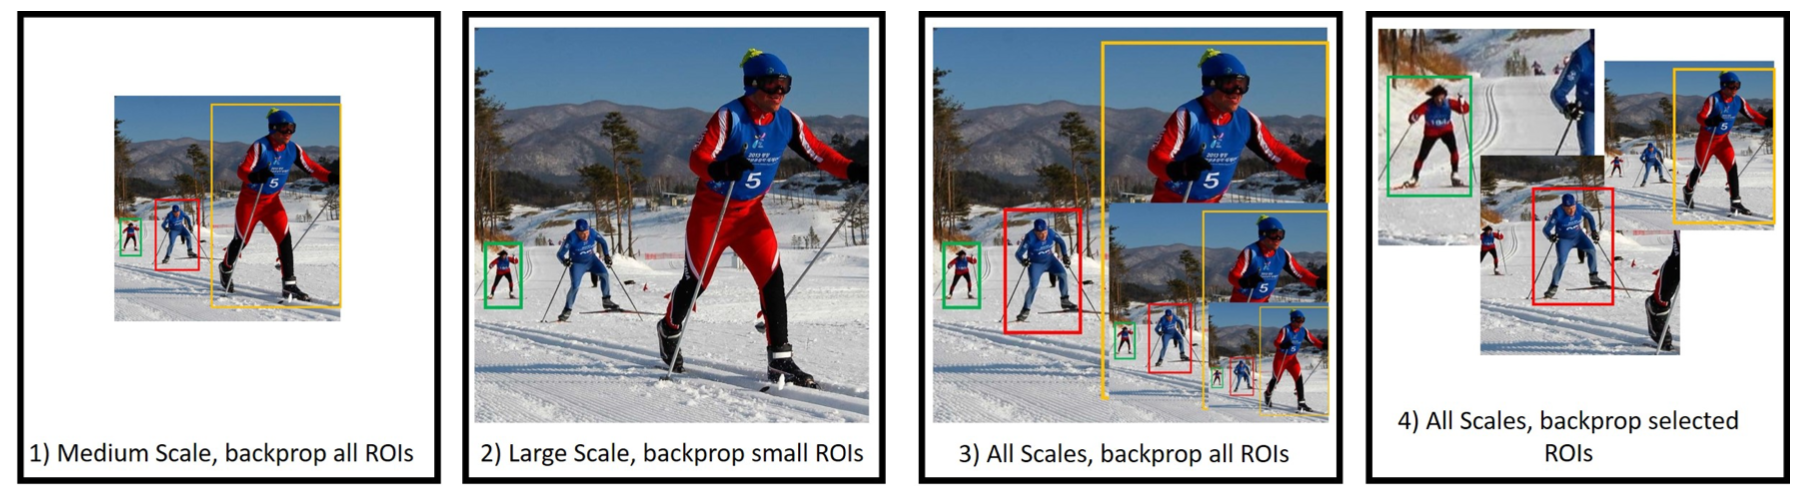
\includegraphics[width=15cm] {images/snip_model_compare}
        \caption{Các cách huấn luyện mô hình khác nhau 1. ${800}_{all}$, 2. ${1400}_{<80px}$, 3. MST, 4. SNIP (Nguồn: \cite{singh2018analysis})}
        \label{fig:snip_model_compare}
    \end{figure}

    \noindent
    Tiếp theo, nhóm tác giả thực hiện \textit{Thí nghiệm huấn luyện mô hình với các đối tượng có kích thước cụ thể}.
    Trong thí nghiệm này, nhóm tác giả vẫn huấn luyện mô hình với bộ dữ liệu có kích thước 1400x2000.
    Tuy nhiên, nhóm tác giả loại bỏ hoàn toàn các đối tượng trung bình và lớn (các đối tượng có kích thước lớn hơn 80 trong ảnh gốc) và gọi là ${1400}_{<80px}$ \\
    \textbf{Kết quả}:
    Kết quả của ${1400}_{<80px}$ rất tệ so với kết quả của ${800}_{all}$ và ${1400}_{all}$. \\
    \textbf{Kết luận}:
    Việc loại bỏ hoàn toàn các đối tượng trung bình và lớn khiến cho lượng dữ liệu mà ${1400}_{<80px}$ được học giảm đi rất nhiều so với các mô hình trên (giảm khoảng 30\% lượng biến thể của đối tượng).
    Từ đó, kết quả của ${1400}_{<80px}$ bị ảnh hưởng nghiêm trọng.
    Chúng ta cũng có thể rút ra được một kết luận là, cho dù các ${1400}_{all}$ và ${800}_{all}$ không hoàn toàn học được các đối tượng trung bình và lớn nhưng lượng dữ liệu từ các đối tượng này vẫn đóng vai trò quan trọng trong việc giúp các mô hình xác định các đối tượng nhỏ.

    \begin{figure}[H]
        \centering
        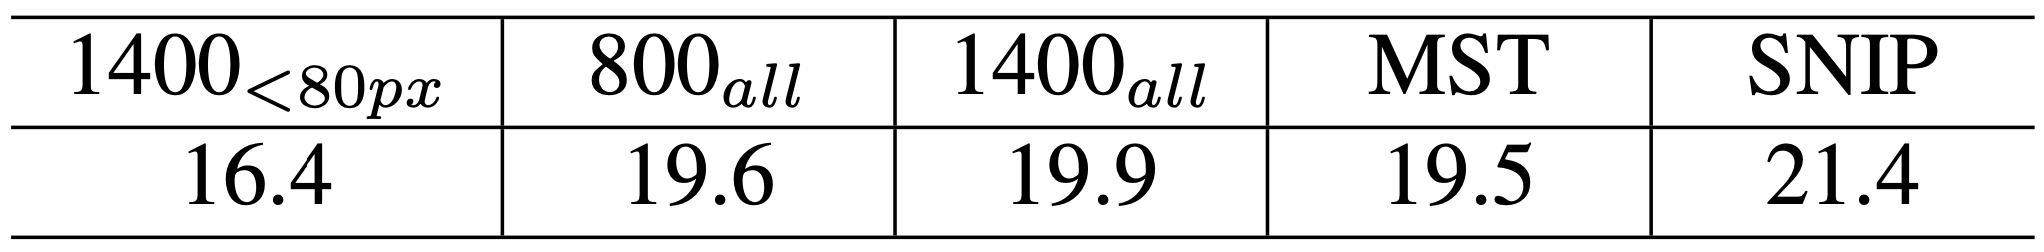
\includegraphics[width=13cm] {images/snip_results_1}
        \caption{So sánh kết quả trên chỉ số mAP của các mô hình ${1400}_{<80px}$, ${800}_{all}$, ${1400}_{all}$, MST và SNIP trên các đối tượng có kích thước nhỏ (nhỏ hơn 32x32) (Nguồn: \cite{singh2018analysis})}
        \label{fig:snip_results_1}
    \end{figure}

    \noindent
    Cuối cùng, nhóm tác giả thực hiện \textit{Thí nghiệm huấn luyện với bộ dữ liệu ảnh có các kích thước khác nhau}.
    Nhóm tác giả huấn luyện mô hình với bộ dữ liệu ảnh có các kích thước khác nhau được lựa chọn ngẫu nhiên trong suốt quá trình huấn luyện (Multi-Scale Training) và gọi đó là MST.
    Thí nghiệm này giúp mô hình có thể được học các kích thước khác nhau với mỗi đối tượng trong bộ dữ liệu. \\
    \textbf{Kết quả}:
    Kết quả của MST xấp xỉ so với kết quả của ${800}_{all}$. \\
    \textbf{Kết luận}:
    Việc chuẩn bị dữ liệu ảnh có các kích thước khác nhau như MST khiến mô hình gặp khó khăn trong việc học các đối tượng rất lớn hoặc rất nhỏ.
    Điều này phần nào đó tương tự với hiện tượng mà ${1400}_{all}$ gặp phải.
}